\documentclass[aspectratio=169,usenames,dvipsnames]{beamer}


\usetheme{default}  % You can choose any other theme you prefer

\title{09 - Algoritmos}
\subtitle{Árvore Geradora Mínimas}
\author{Mateus Oliveira de Figueiredo}
\date{21/11/2023}

\usepackage{tikz}
\usetikzlibrary{matrix}
\usepackage{multicol}
\usepackage{algorithm}
\usepackage{algpseudocode}
\usepackage{xcolor}
\usepackage[utf8]{inputenc}
\usepackage[portuguese]{babel}
\usepackage{amsmath} % for "pmatrix" environment  
\usepackage{pgffor} 
\usepackage{listings}

\usepackage{pgfplots}
\DeclareUnicodeCharacter{2212}{−}
\usepgfplotslibrary{groupplots,dateplot}
\usetikzlibrary{patterns,shapes.arrows, positioning, arrows}
\usetikzlibrary{graphs, graphs.standard}
\pgfplotsset{compat=newest}

\lstset{
  language=Python,
  basicstyle=\ttfamily\tiny,
  keywordstyle=\color{blue},
  commentstyle=\color{green},
  stringstyle=\color{red},
  stepnumber=1,
  numbersep=10pt,
  showspaces=false,
  showstringspaces=false,
  tabsize=2,
  breaklines=true,
  breakatwhitespace=true,
}

\begin{document}

\begin{frame}
\titlepage
\end{frame}

\begin{frame}
\frametitle{Árvores Geradoras Mínimas}

Árvore geradora que possui a menor soma de pesos das arestas.

\vfill
Algoritmos:
\begin{itemize}
  \item Algoritmo de Prim
  \item Algoritmo de Kruskal
\end{itemize}
\vfill
\end{frame}


\begin{frame}
\frametitle{Proposição Aresta de Cruzamento}

\vfill
\begin{block}{Proposição}
    Dado um corte em um grafo a aresta de cruzamento de menor peso está na árvore geradora mínima.
\end{block}
\vfill

\begin{columns}
\column{0.5\textwidth}

\begin{figure}[ht]
\centering
\includegraphics[width=0.5\textwidth]{figs/prim.png}
\caption{Prim\footnote{Algorithms Fourth Edition: Sedgewick, Wayne}}
\end{figure}
\column{0.5\textwidth}

\begin{figure}[ht]
\centering
\includegraphics[width=0.5\textwidth]{figs/kruskal.png}
\caption{Kruskal $^\text{a}$}
\end{figure}
\end{columns}
\vfill

% Add footnote with figures source


\end{frame}


\begin{frame}{Union Find}
    Estrutura de Dados para representar conjuntos disjuntos.

    \begin{itemize}
        \item Find: Encontrar o representante do conjunto
        \item Union: Unir dois conjuntos
    \end{itemize}

\begin{tikzpicture}[scale=0.75, transform shape, node distance=1.5cm]
    % Style for the circles
    \tikzstyle{circle node}=[circle, draw, minimum size=1cm]

    % Draw the top array boxes and numbers
    \foreach \x in {0,...,6}
        \draw (\x-1,0) rectangle (\x+0,-0.5) node[pos=.5] {\x};
    \foreach \x/\num in {0/0,1/0,2/0,3/3,4/3,5/3,6/5}
        \draw (\x-1,-0.5) rectangle (\x+0,-1) node[pos=.5] {\num};

    % Draw the circles for the tree
    \node[circle node] (0) at (0,2) {0};
    \node[circle node] (1) at (-1,1) {1};
    \node[circle node] (2) at (1,1) {2};
    \node[circle node] (3) at (4,2) {3};
    \node[circle node] (4) at (3,1) {4};
    \node[circle node] (5) at (5,1) {5};
    \node[circle node] (6) at (6,0) {6};

    % Draw the arrows for the tree
    \draw[->] (1) -- (0);
    \draw[->] (2) -- (0);
    \draw[->] (4) -- (3);
    \draw[->] (5) -- (3);
    \draw[->] (6) -- (5);

    % Repeat the process for the bottom part with different positions
    % and arrows indicating values have been moved
    
    % Additional nodes and arrows would go here...

\end{tikzpicture}
\end{frame}

\begin{frame}{Exemplo Pequeno - Prim}
    \begin{columns}
    \column{0.5\textwidth}
    \begin{figure}[ht]
    \centering
        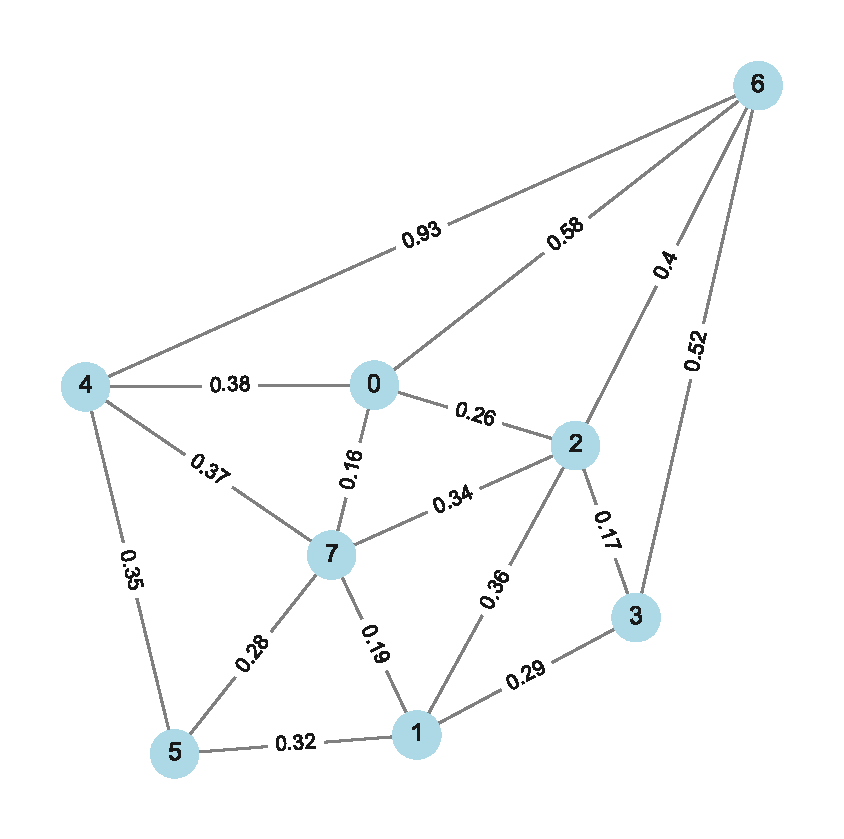
\includegraphics[width=0.9\textwidth]{figs/exemplo_0.pdf}
    \end{figure}
    \column{0.5\textwidth}
        \begin{figure}[ht]
        \centering
            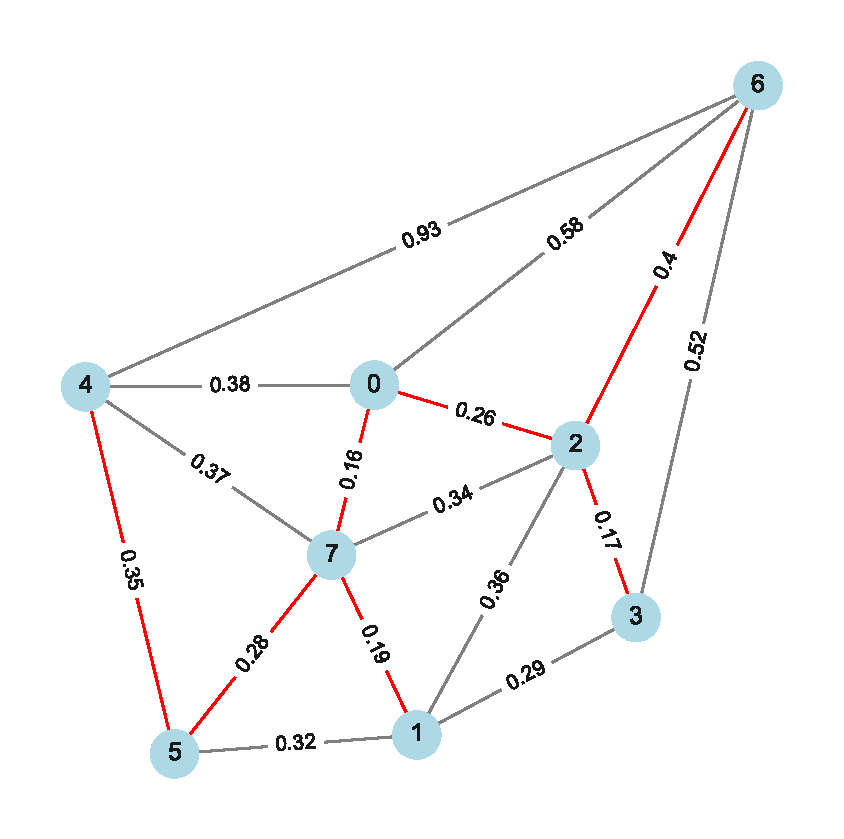
\includegraphics[width=0.9\textwidth]{figs/exemplo_0_prim.pdf}

        \end{figure}
    \end{columns}
\end{frame}

\begin{frame}{Exemplo Pequeno - Kruskal}
    \begin{columns}
    \column{0.5\textwidth}
    \begin{figure}[ht]
    \centering
        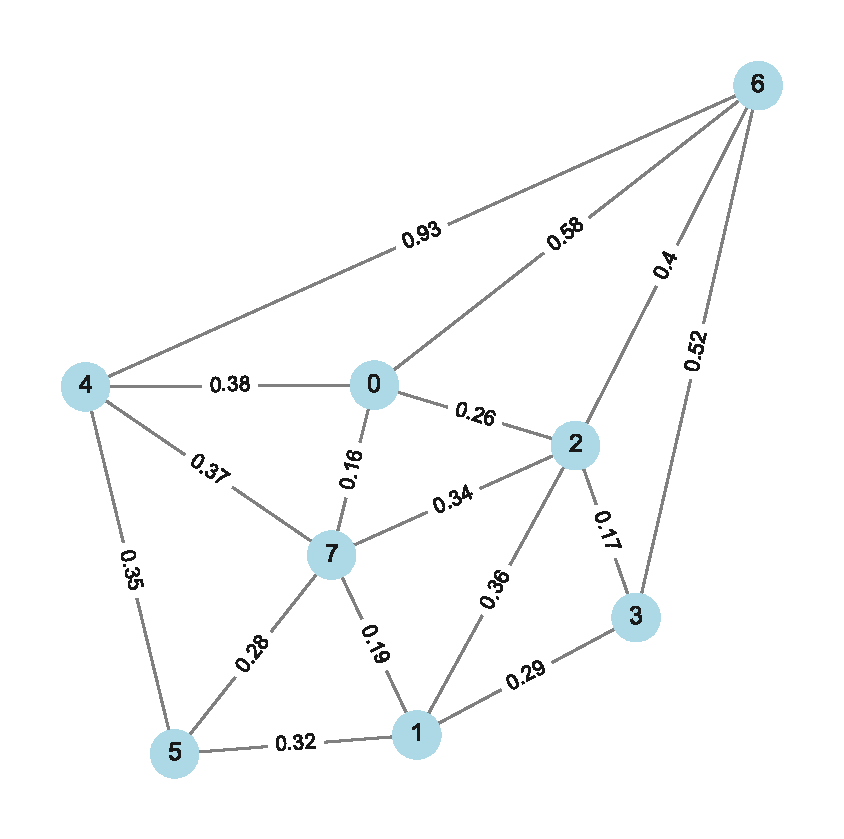
\includegraphics[width=0.9\textwidth]{figs/exemplo_0.pdf}
    \end{figure}
    \column{0.5\textwidth}
        \begin{figure}[ht]
        \centering
            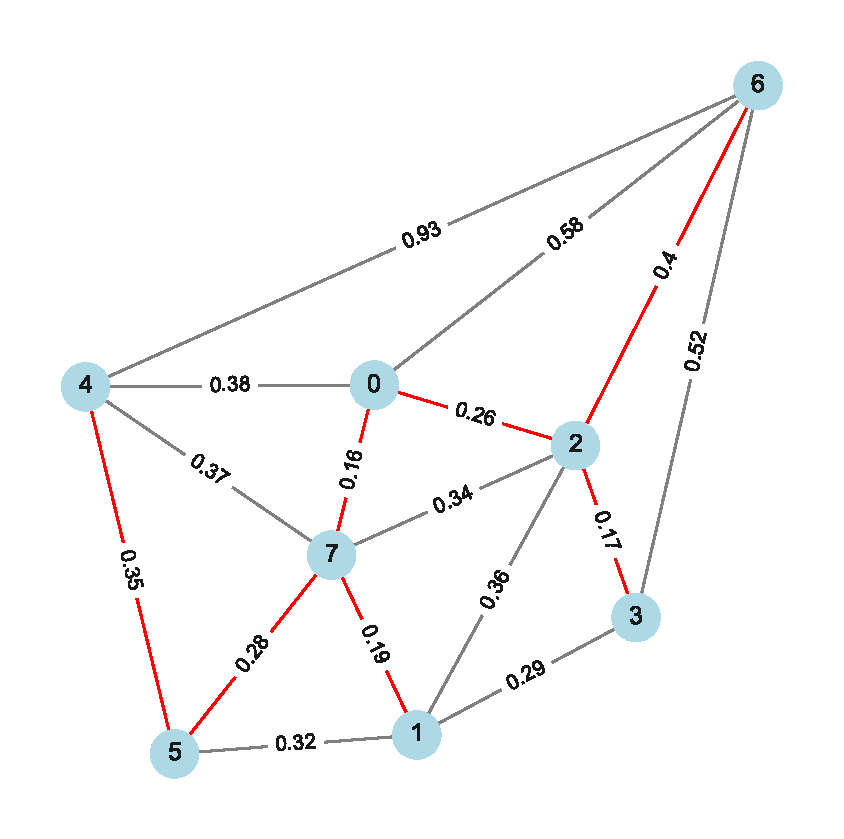
\includegraphics[width=0.9\textwidth]{figs/exemplo_0_kruskal.pdf}
        \end{figure}
    \end{columns}
\end{frame}


\foreach \i in {28, 56, 138, 221, 249} {
    \begin{frame}{Exemplo Médio - Prim x Kruskal}
        \begin{columns}
        \column{0.5\textwidth}
        \begin{figure}[ht]
        \centering
            \includegraphics[width=0.9\textwidth]{figs/mediumewg/prim_step_\i.pdf}
        \end{figure}
        \column{0.5\textwidth}
            \begin{figure}[ht]
            \centering
                \includegraphics[width=0.9\textwidth]{figs/mediumewg/kruskal_step_\i.pdf}
            \end{figure}
        \end{columns}
    \end{frame}
}

\begin{frame}{Performance dos Algoritmos}

    \begin{columns}
    \column{0.4\textwidth}

    \begin{itemize}
        \item Completo: m = n(n-1)/2
        \item m = 2n
    \end{itemize}
    
    \column{0.6\textwidth}
        \begin{figure}[ht]
            \centering
            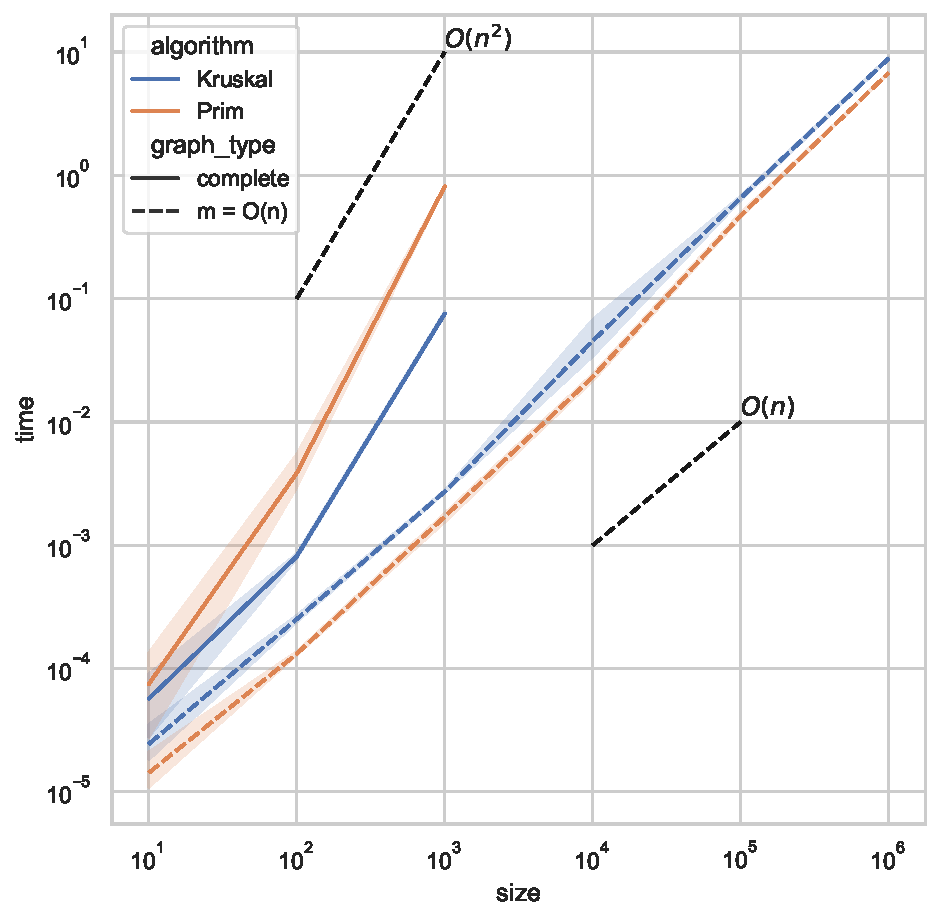
\includegraphics[width=0.8\textwidth]{figs/complexity.pdf}
        \end{figure}
    \end{columns}
    
\end{frame}


\begin{frame}{Resultados com Dados da Anac}

    \vfill
    \begin{itemize}
        \item Realizado testes com dados da ANAC
        \item Bibliotecas: geopandas e geopy
        \item Peso das arestas como mediana da duração do voo ou distância (geodésia)
        \item Removido voos cancelados ou com duração negativa
    \end{itemize}
    \vfill
\end{frame}

\begin{frame}{Prim x Kruskal - Duração do Voo}
    \begin{figure}[ht]
        \centering
        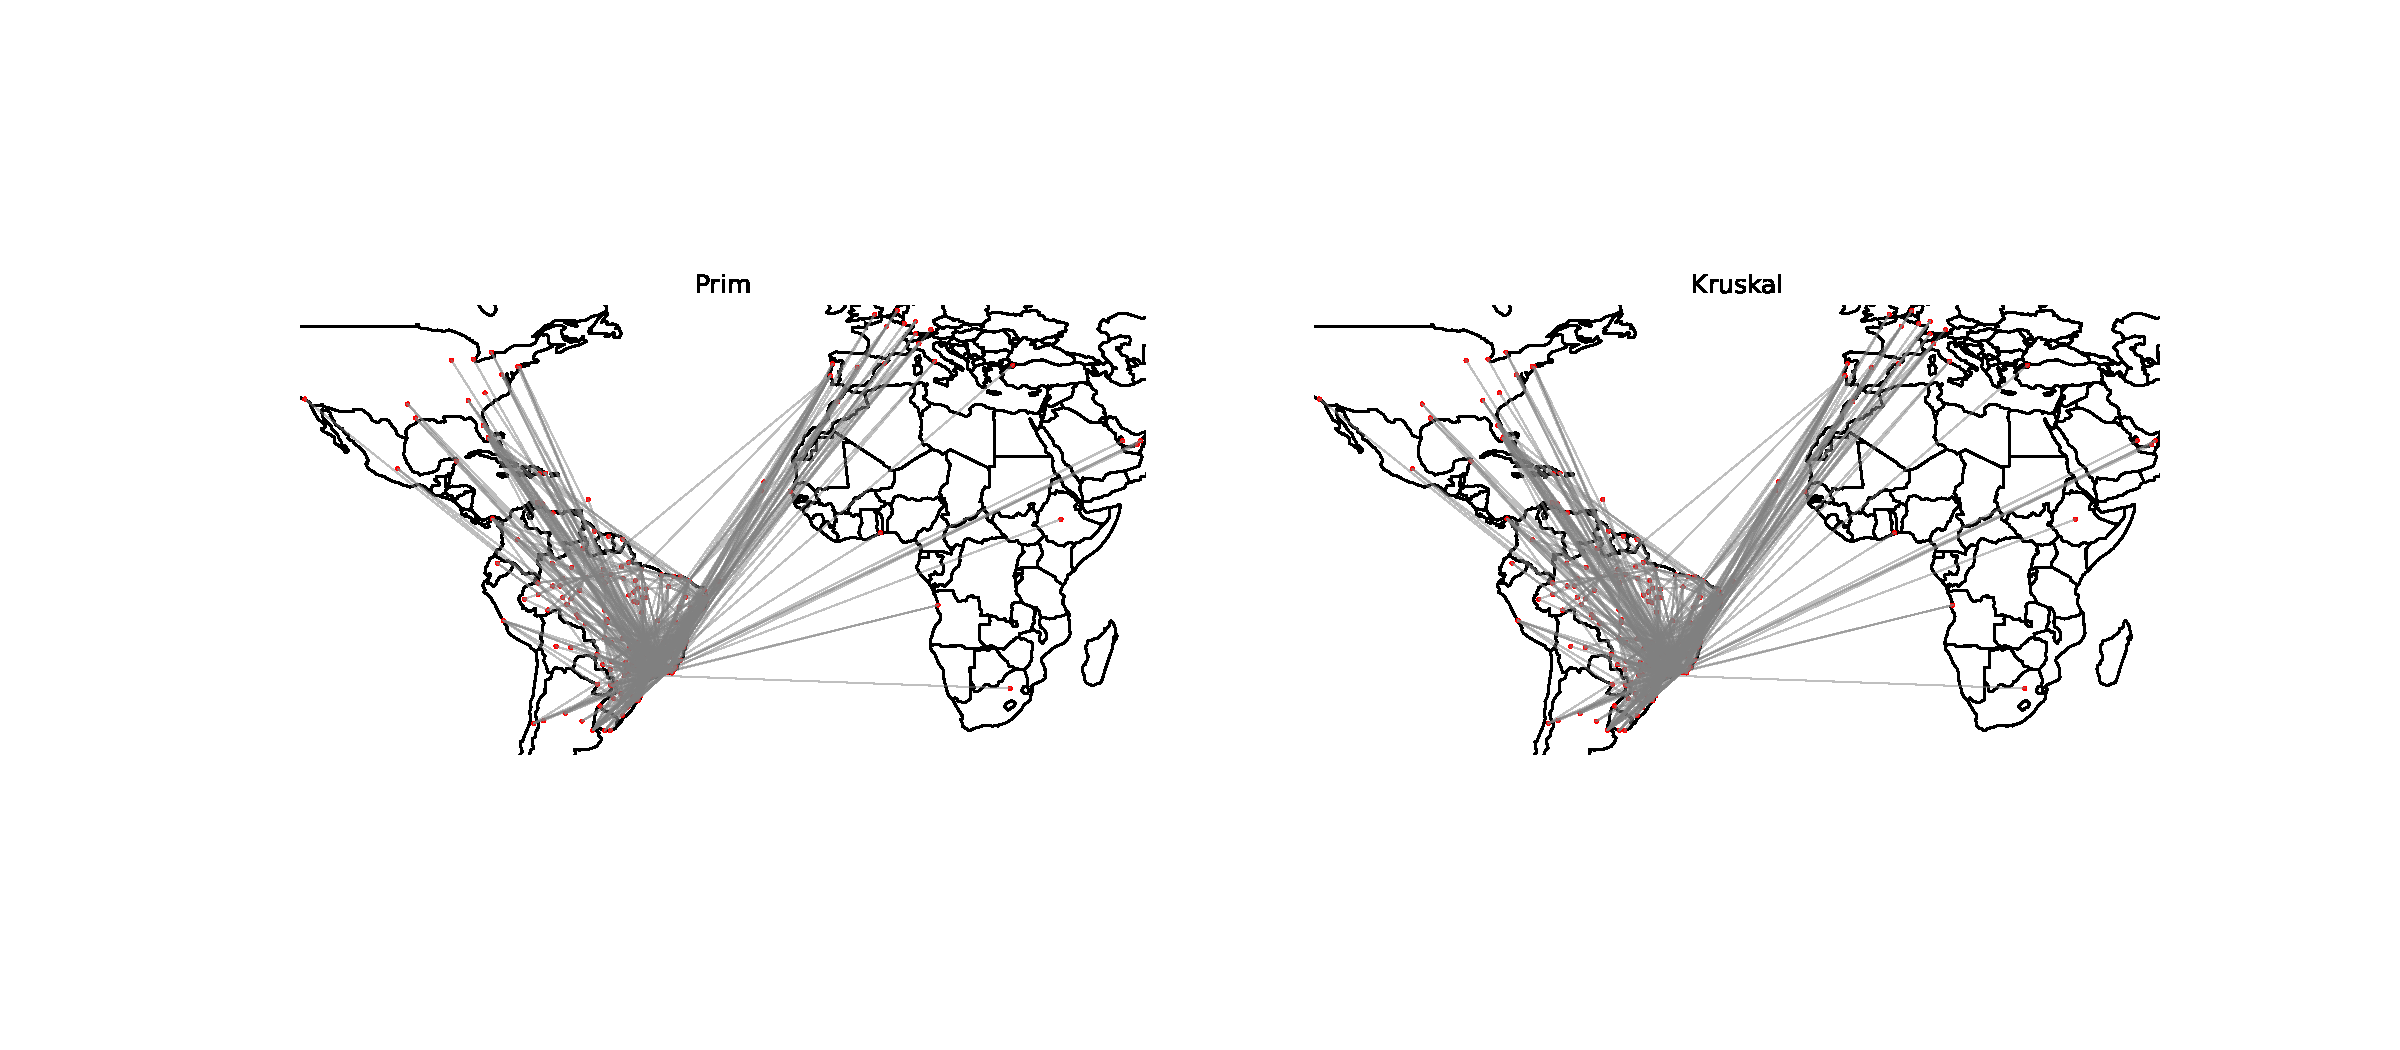
\includegraphics[width=\textwidth]{figs/world_time_mst_0.pdf}
    \end{figure}
\end{frame}

\begin{frame}{Prim x Kruskal - Duração do Voo}
    \begin{figure}[ht]
        \centering
        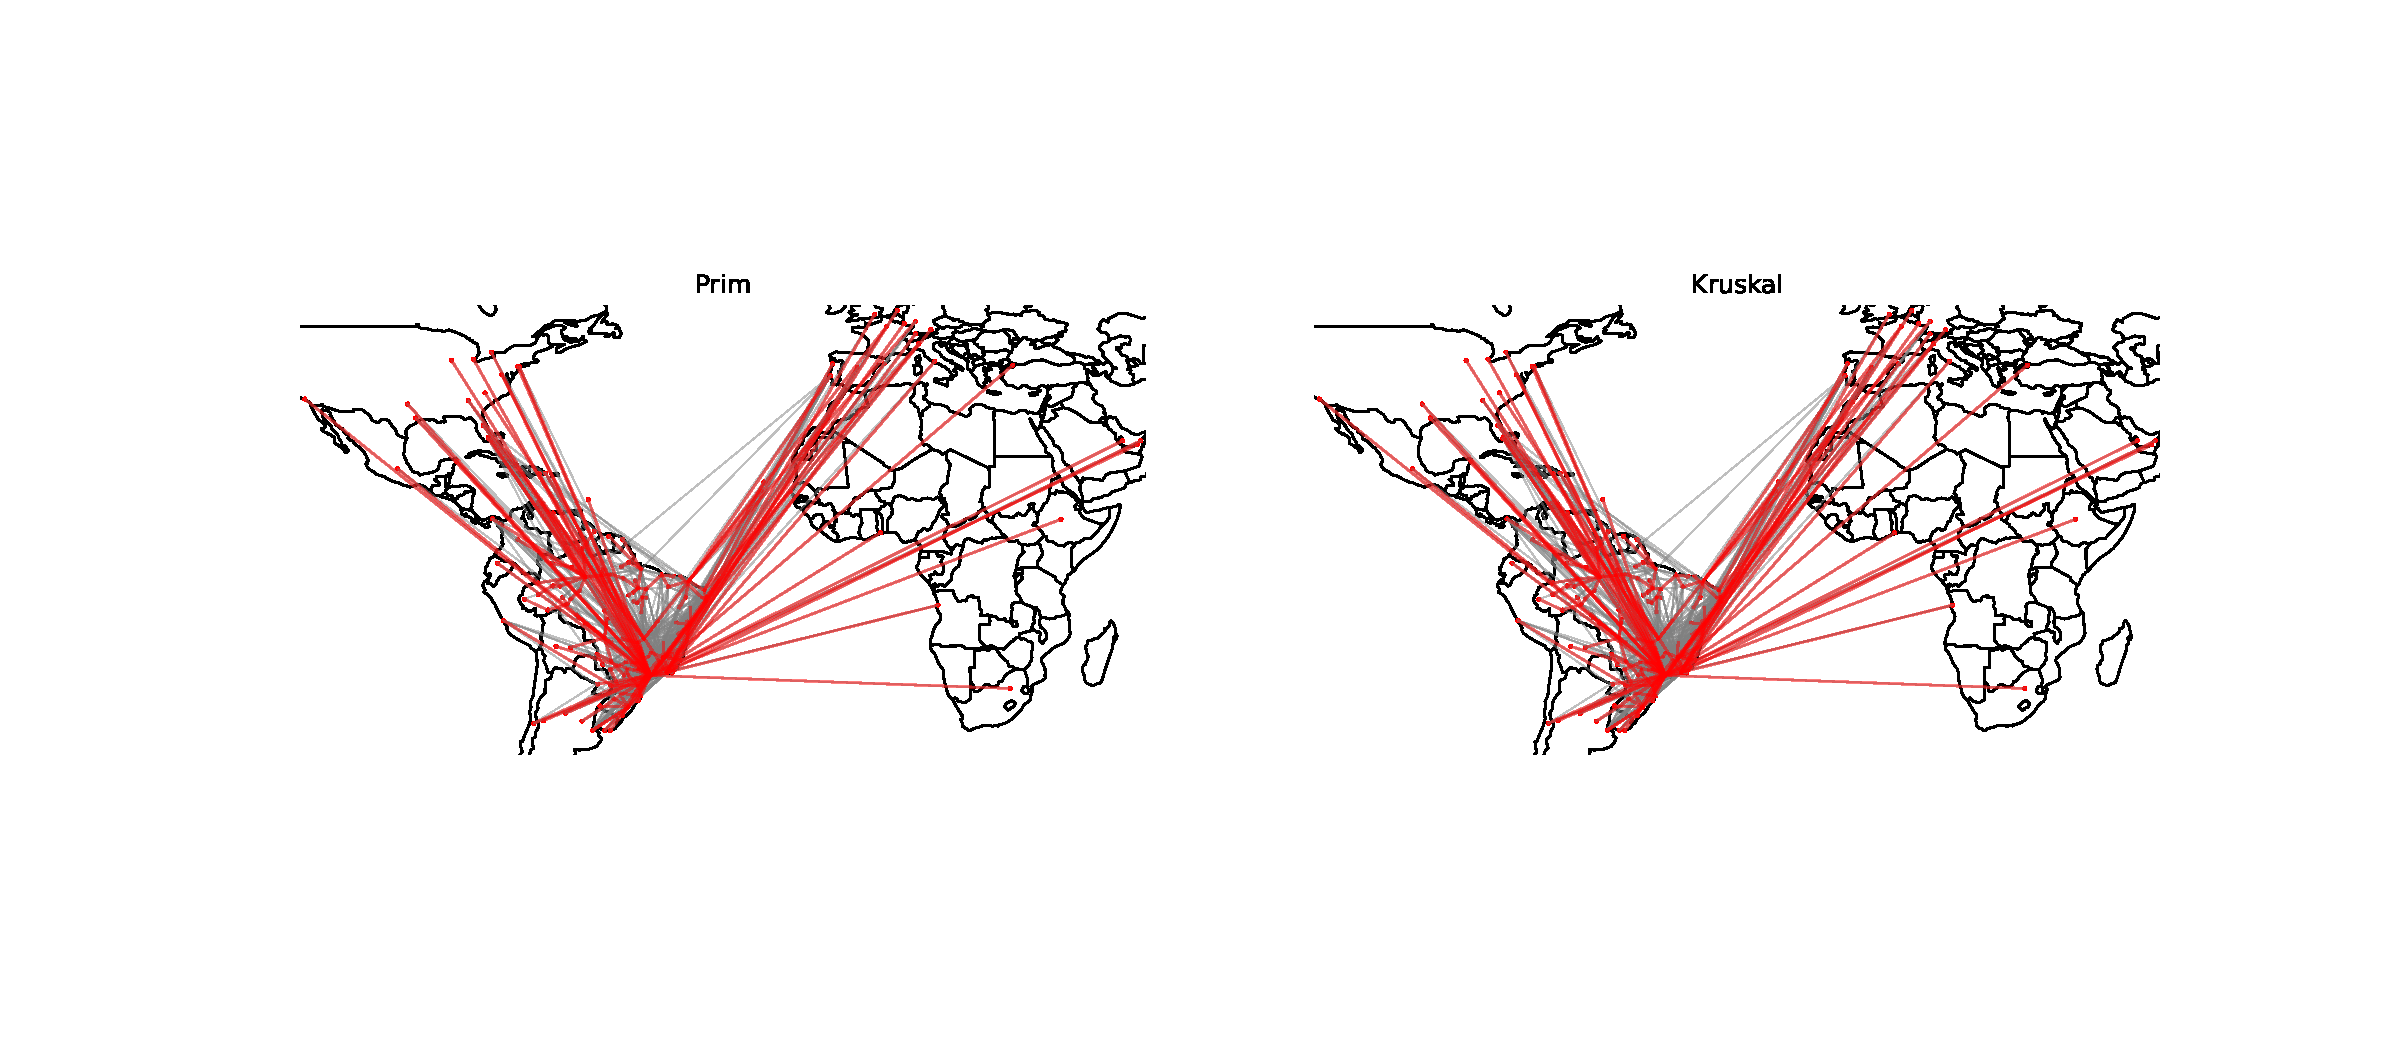
\includegraphics[width=\textwidth]{figs/world_time_mst_1.pdf}
    \end{figure}
\end{frame}

\begin{frame}{Prim x Kruskal - Duração do Voo - Brasil}
    \begin{figure}[ht]
        \centering
        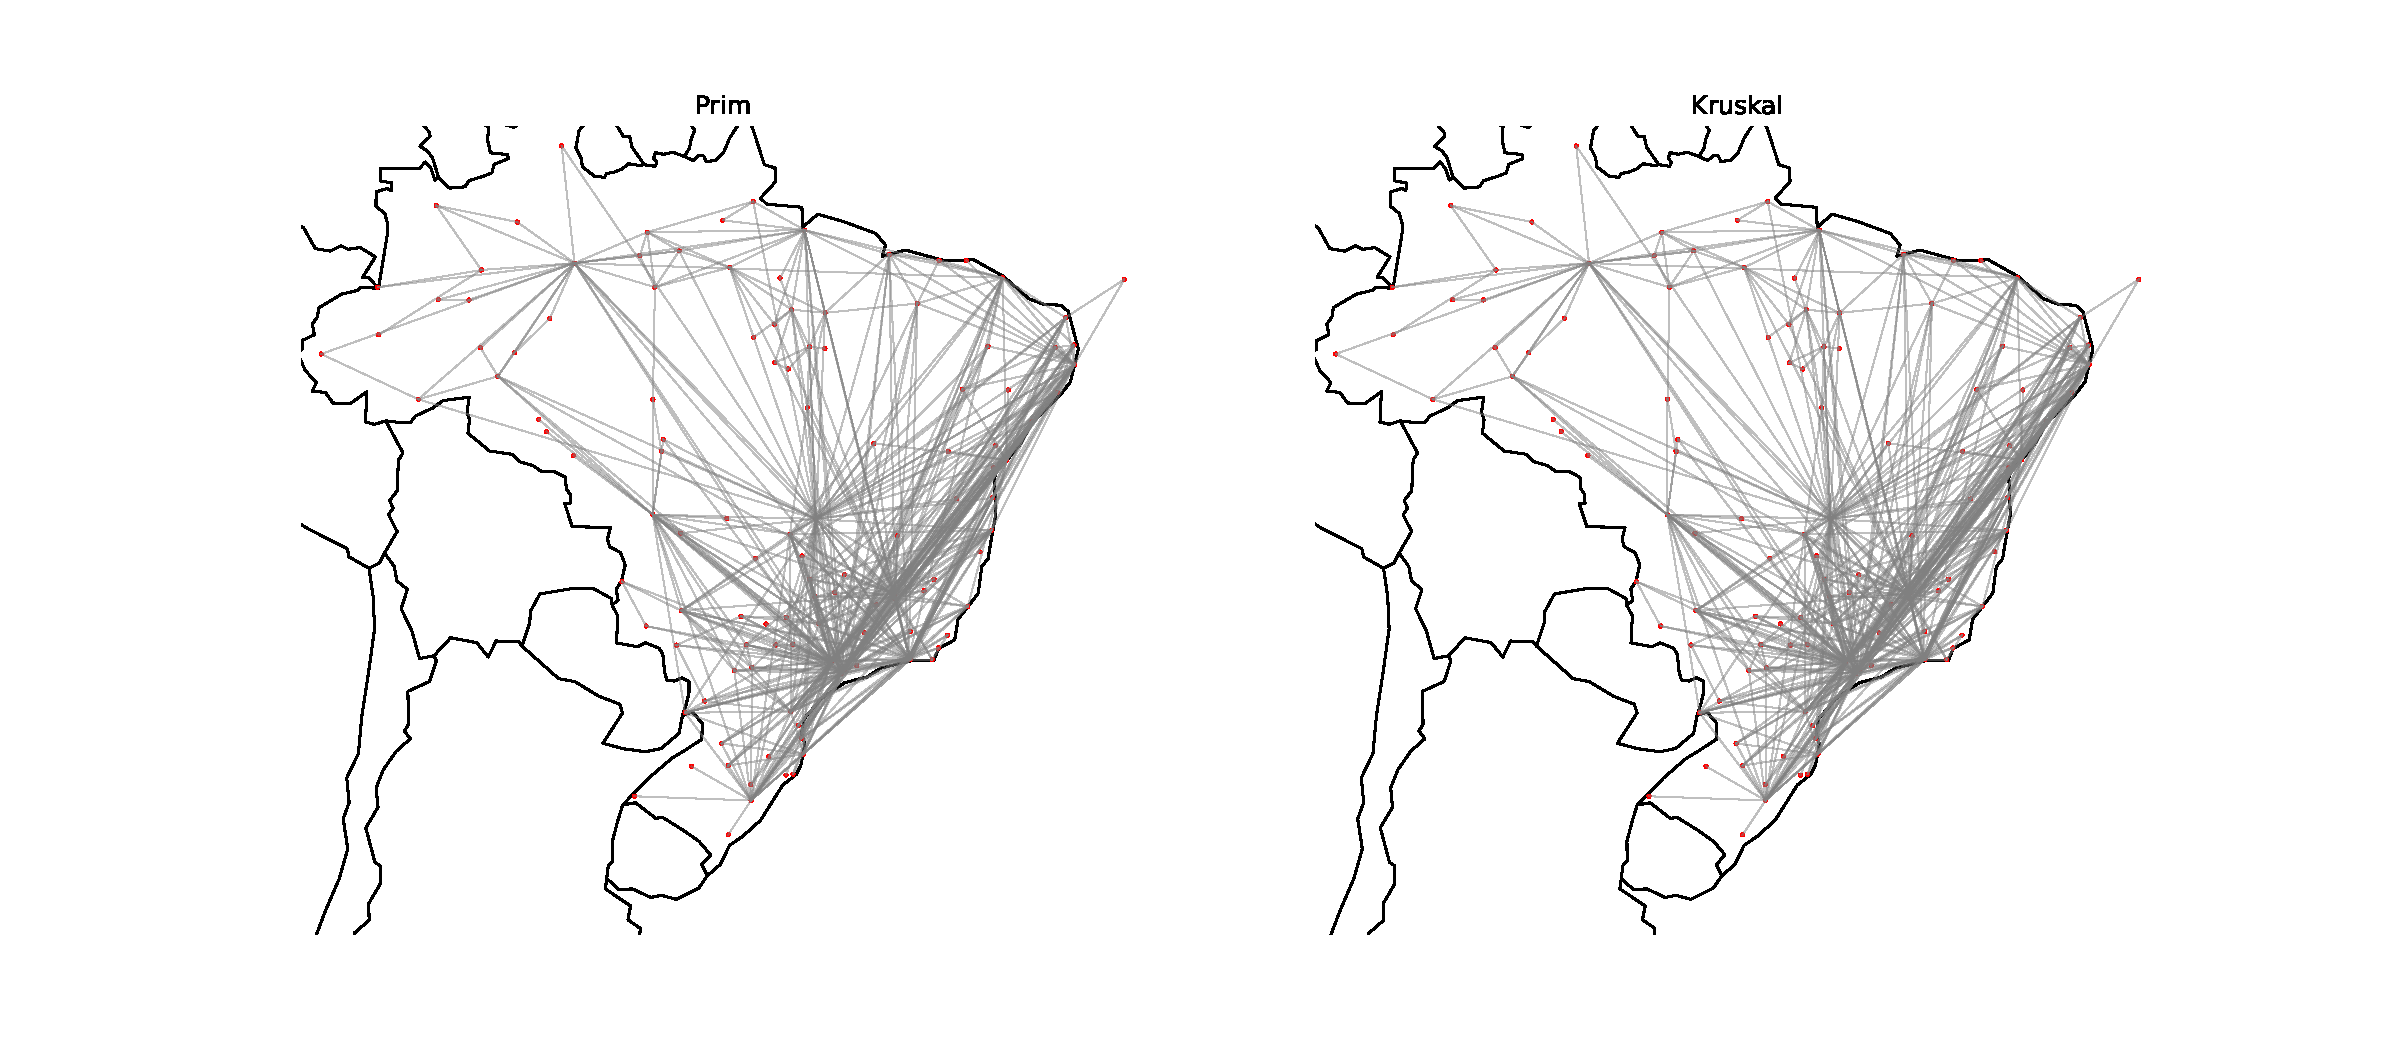
\includegraphics[width=\textwidth]{figs/brasil_time_mst_0.pdf}
    \end{figure}
\end{frame}

\begin{frame}{Prim x Kruskal - Duração do Voo - Brasil}
    \begin{figure}[ht]
        \centering
        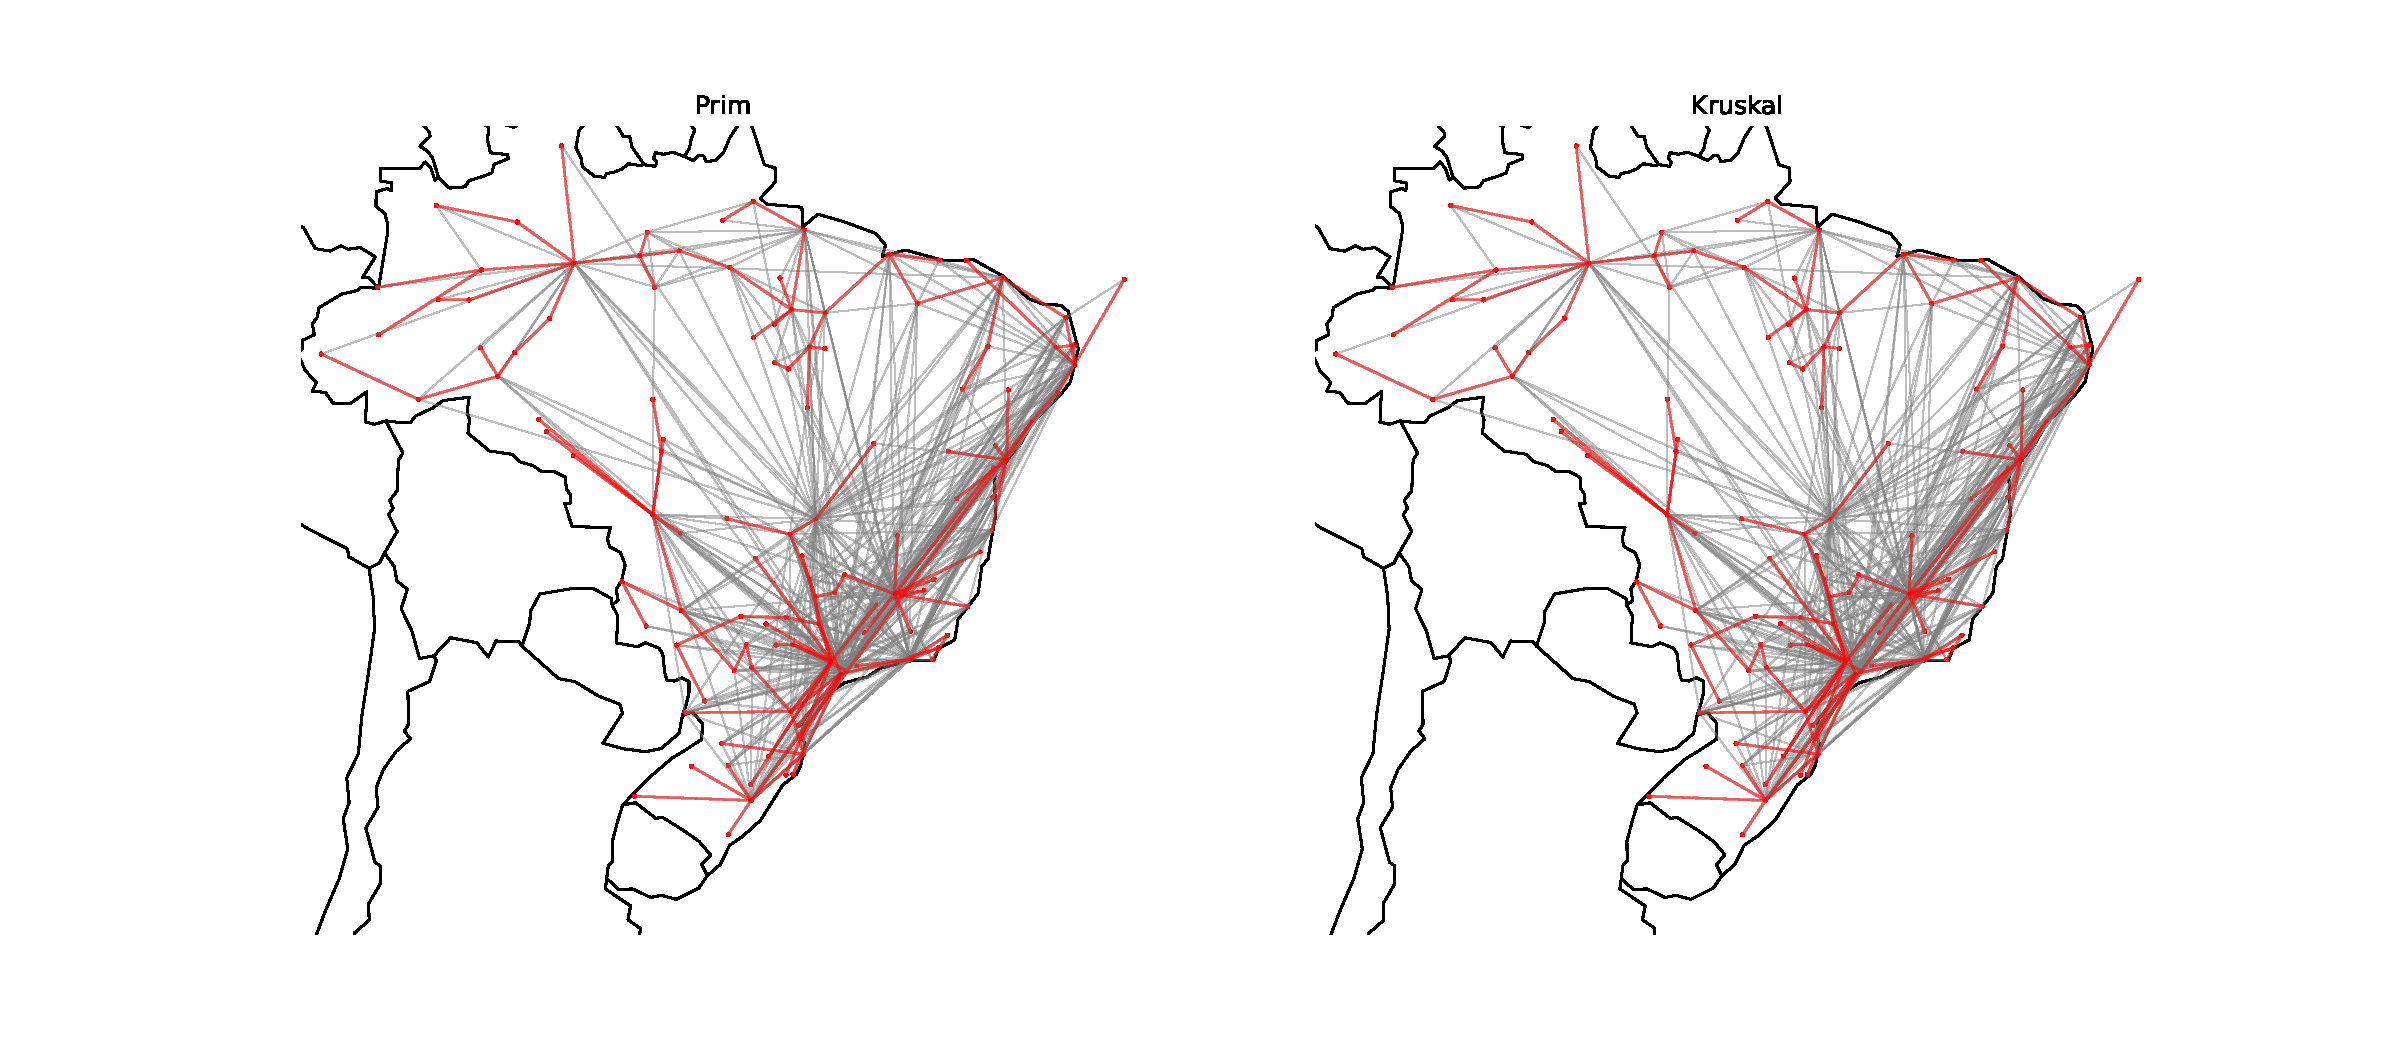
\includegraphics[width=\textwidth]{figs/brasil_time_mst_1.pdf}
    \end{figure}
\end{frame}

\begin{frame}{Duração x Distância - Brasil}
    \begin{figure}[ht]
        \centering
        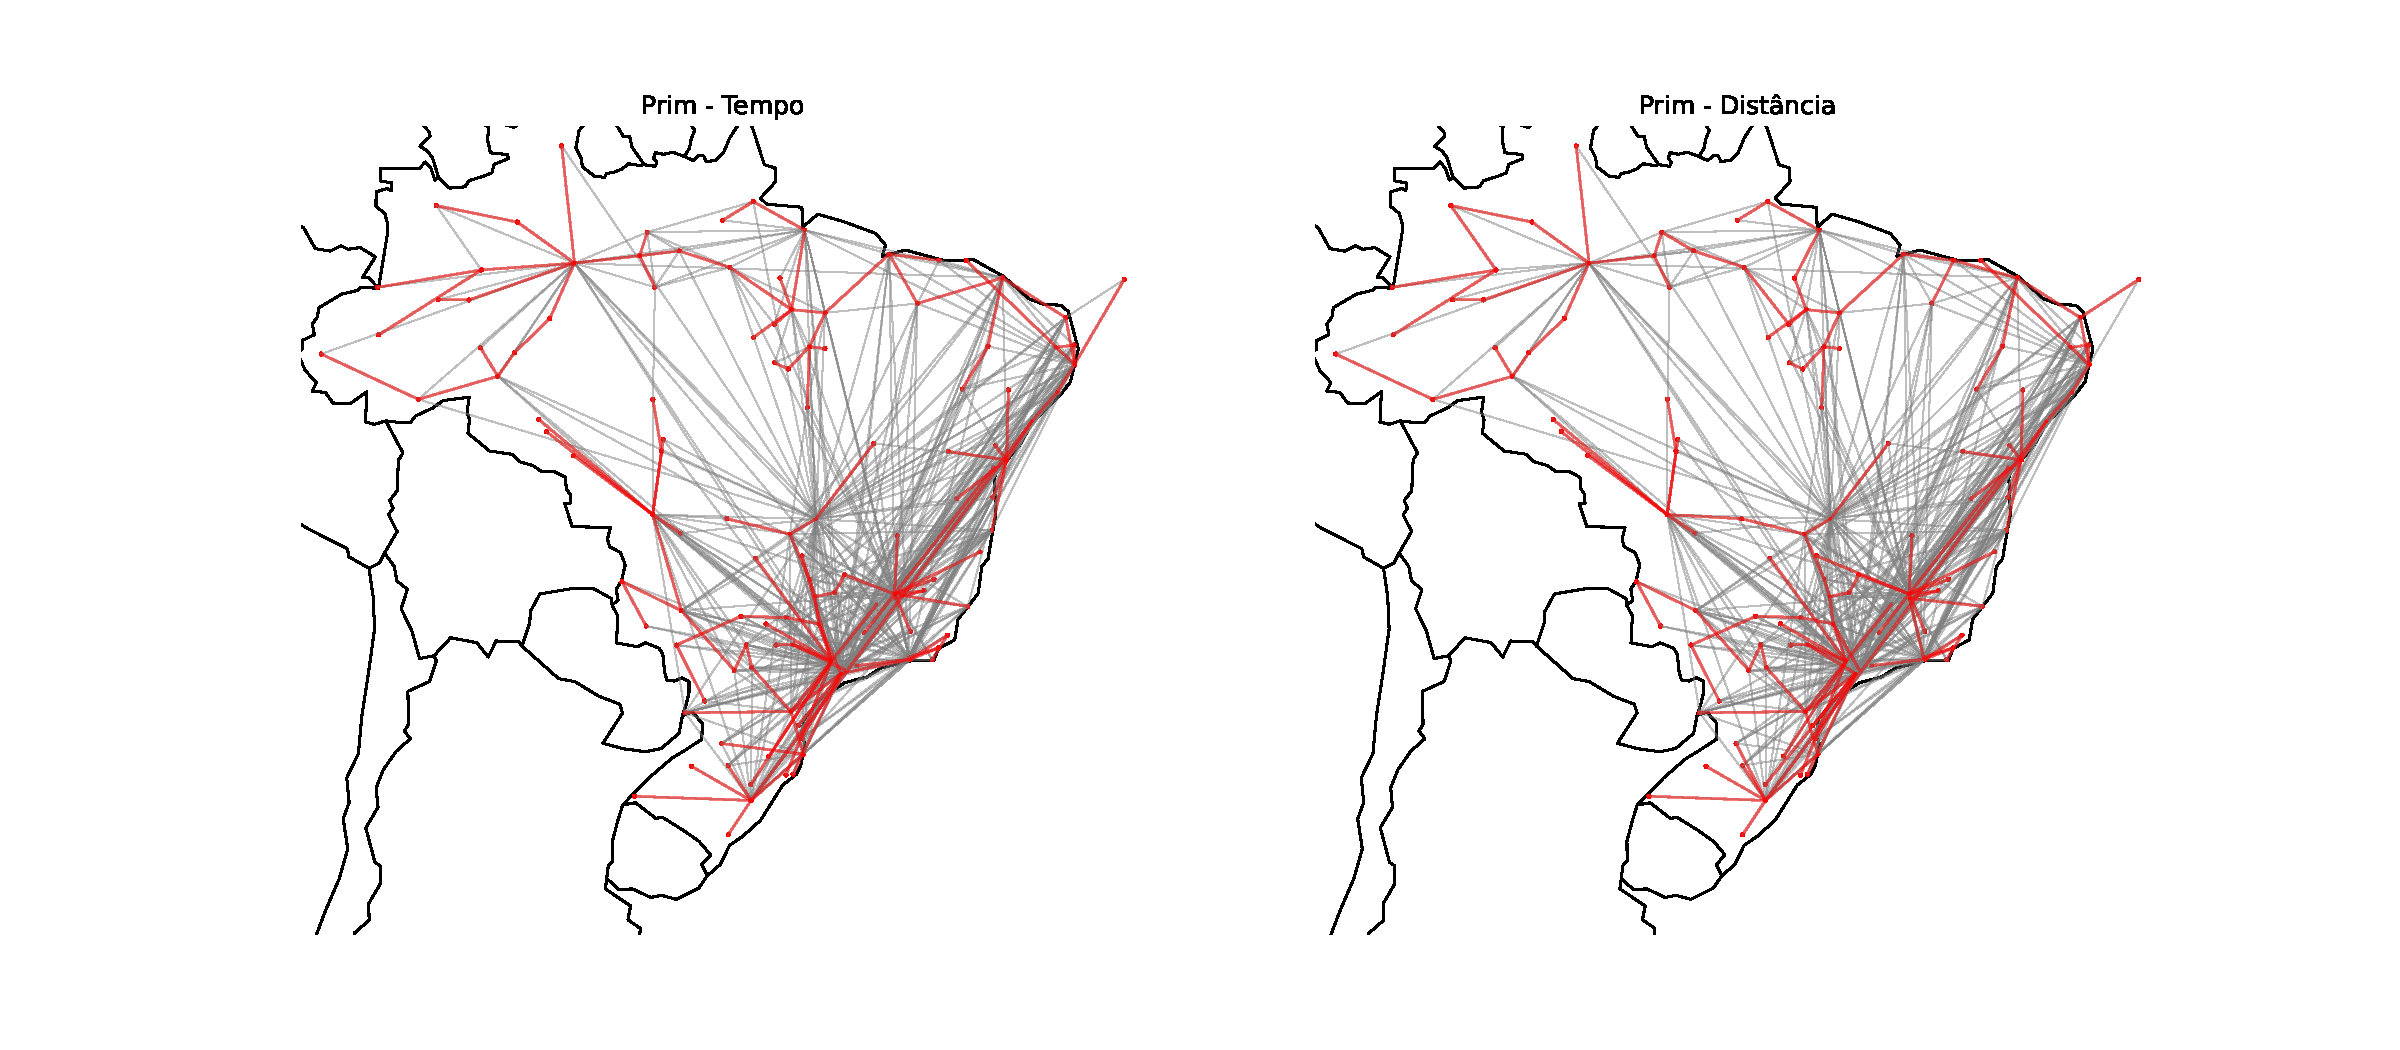
\includegraphics[width=\textwidth]{figs/brasil_time_x_distance_mst_1.pdf}
    \end{figure}
\end{frame}

\begin{frame}{Duração x Distância - Fernando de Noronha}
    \begin{figure}[ht]
        \centering
        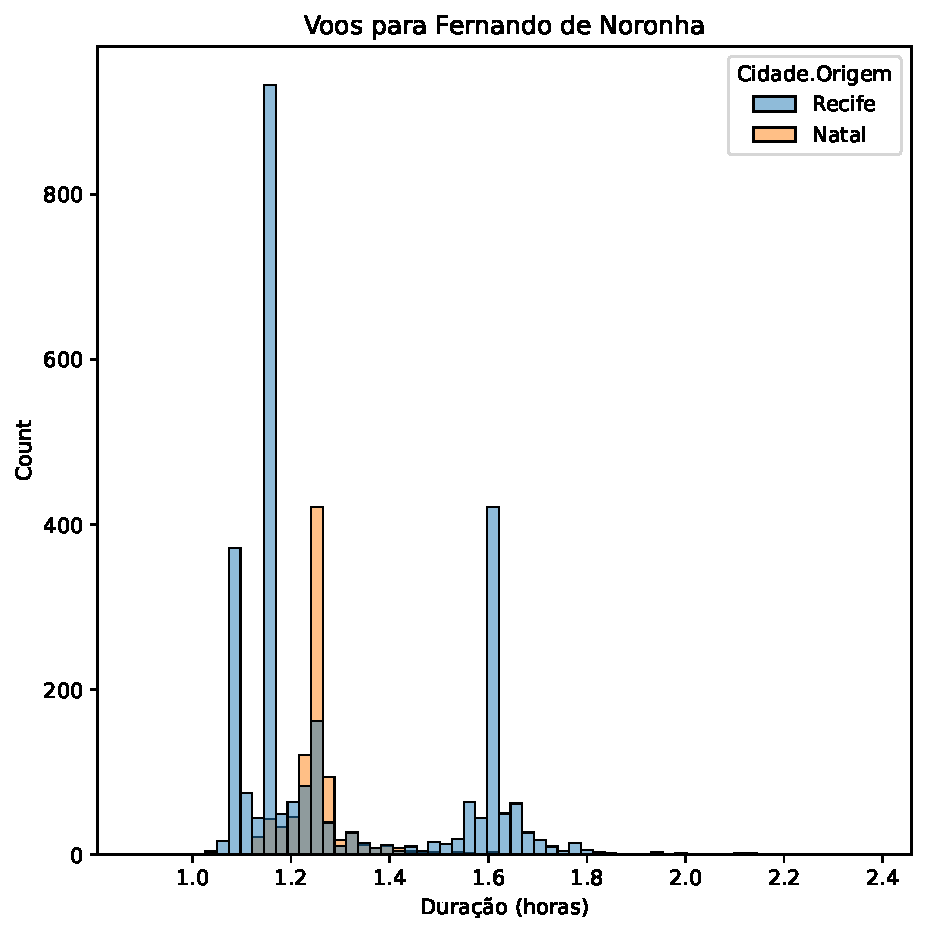
\includegraphics[width=0.5\textwidth]{figs/histograma_fernando_noronha.pdf}
    \end{figure}
\end{frame}


\end{document}
